\documentclass[a4paper,12pt]{report}
\usepackage{graphicx}
\usepackage{hyperref}
\usepackage[spanish]{babel}
\usepackage{fancyhdr}
\usepackage{tocloft}
\usepackage{setspace}
\usepackage{ragged2e}
% Permite el uso de títulos, encabezados y pies de página.
\usepackage{titlesec}
% Permite la inserción de imágenes al archivo.
\usepackage{graphicx}
% Permite el uso de imágenes y figuras rotadas
\usepackage{rotating}
% Permite cambiar el tamaño de las imágenes.
\usepackage[export]{adjustbox}
% Permite el uso de hojas apaisadas y verticales.
\usepackage{pdflscape}
% Permite el uso de múltiples imágenes dentro de una figura.
\usepackage{subcaption}
% Permite la definición de objetos flotantes como tablas e imágenes.
\usepackage{float}
% Expande las capacidades de las tablas.
\usepackage{array}
% Expande las capacidades de las tablas.
\usepackage{tabularray}
\usepackage{appendix}
\usepackage{tabularx}% Permite el uso de ítems con diferente forma.
\usepackage{enumitem}
\usepackage{xcolor} % Asegúrate de incluir este paquete
\definecolor{Celeste}{HTML}{00B5BE} % Reemplaza '00B5BE' por el código que desees

% Configuración de márgenes y encabezados
\usepackage[a4paper, margin=2.5cm]{geometry}
\pagestyle{fancy}
\fancyhf{}
\fancyhead[L]{Rev-Control}
\fancyhead[R]{\leftmark}
\fancyfoot[C]{\thepage}

% Establece que en la tabla de contenidos se use una línea de puntos para marcar el número de página.
\renewcommand{\cftsecleader}{\cftdotfill{\cftdotsep}}

\begin{document}

% Carátula
\begin{titlepage}
    \centering
    % Imagen rectangular grande y estrecha centrada
    \begin{figure}
        \centering
        
\includegraphics[width=1.1\textwidth, height=2.3cm]{Imagenes/logos2.png} % Reemplaza por tu imagen
    \end{figure}
    
    % Logo del proyecto
    
\includegraphics[width=0.7\textwidth]{Imagenes/LOGO REV CONTROL OFICIAL.png} 
    \vspace{1cm}
    
    {\Huge \textbf{\textcolor{Celeste}{Carpeta Técnica}\\}}
    \vspace{1cm}
    {\Large Curso: 7° 1° Aviónica\\}
    \vspace{0.5cm}
    {\Large Comisión: C}
    \vspace{1cm}

    \textbf{Pagina web:} \href{https://www.google.com/}{Link de acceso}\\
    \textbf{Trello:} \href{https://trello.com/b/yDSPDlAp/kanban}{Link de acceso}\\
    \textbf{Github:} \href{https://github.com/impatrq/revcontrol}{Link de acceso}\\
    \textbf{Redes Sociales:} \href{https://www.instagram.com/rev.control/}{Link de acceso} \\
    \vfill
    \textbf{IMPA TRQ E.E.S.T N°7 2024}
\end{titlepage}

%\renewcommand{\contentsname}{Índice general}
\tableofcontents
\newpage

% 2. Presentación del equipo
\chapter{Preámbulo}
    \section{Integrantes}
    
        \begin{itemize}
            \item Gonzalo Acosta
            \item Lautaro Alfaro
            \item Leonardo He
            \item Tadeo Ibaceta
            \item Marcos Martinez
            \item Juan Quintero
            \item Santiago Flores
        \end{itemize}
                    
    
    \section{Foto de cada integrante}
    Información\par
    
    \section{Foto grupal}
    Información\\
    
    \section{Horas dedicadas por cada integrante (registro personal)}
    Información\\
% 4. Introducción
\chapter{Introducción}

\section{Objetivo}  
El objetivo de \textbf{REV-CONTROL} es ofrecer una solución innovadora y accesible para técnicos y mecánicos, permitiendo medir de manera eficiente y precisa los parámetros críticos de un motor. Este banco de prueba portátil, REV-CONTROL, facilita el diagnóstico y mantenimiento, utilizando tecnología de punta de amplificación y filtración de señales para proporcionar datos en tiempo real sobre las condiciones del motor.

\section{Descripción de la solución buscada}  
REV-CONTROL es un banco de prueba portátil diseñado para obtener datos precisos sobre los parámetros esenciales de cualquier motor. Con su diseño compacto y fácil de usar, REV-CONTROL está optimizado para realizar mediciones de revoluciones por minuto (RPM), presión y temperatura del aceite, temperatura de la cabeza de cilindro, temperatura de agua y concentración de oxígeno en los gases. Su sistema permite a los técnicos tomar decisiones rápidas y acertadas para garantizar el correcto funcionamiento de los motores.

\section{Segmento destino y alcance}  
El público objetivo de \textbf{REV-CONTROL} son los técnicos y mecánicos que trabajan en mantenimiento y diagnóstico de motores, desde vehículos de carretera hasta equipos industriales. Con un alcance global, este sistema busca transformar el modo en que se gestionan las pruebas de motor, especialmente en situaciones donde la portabilidad, la rapidez y la precisión son esenciales.

\section{Captura representativa del proyecto}

\begin{figure}[H]
    \centering
    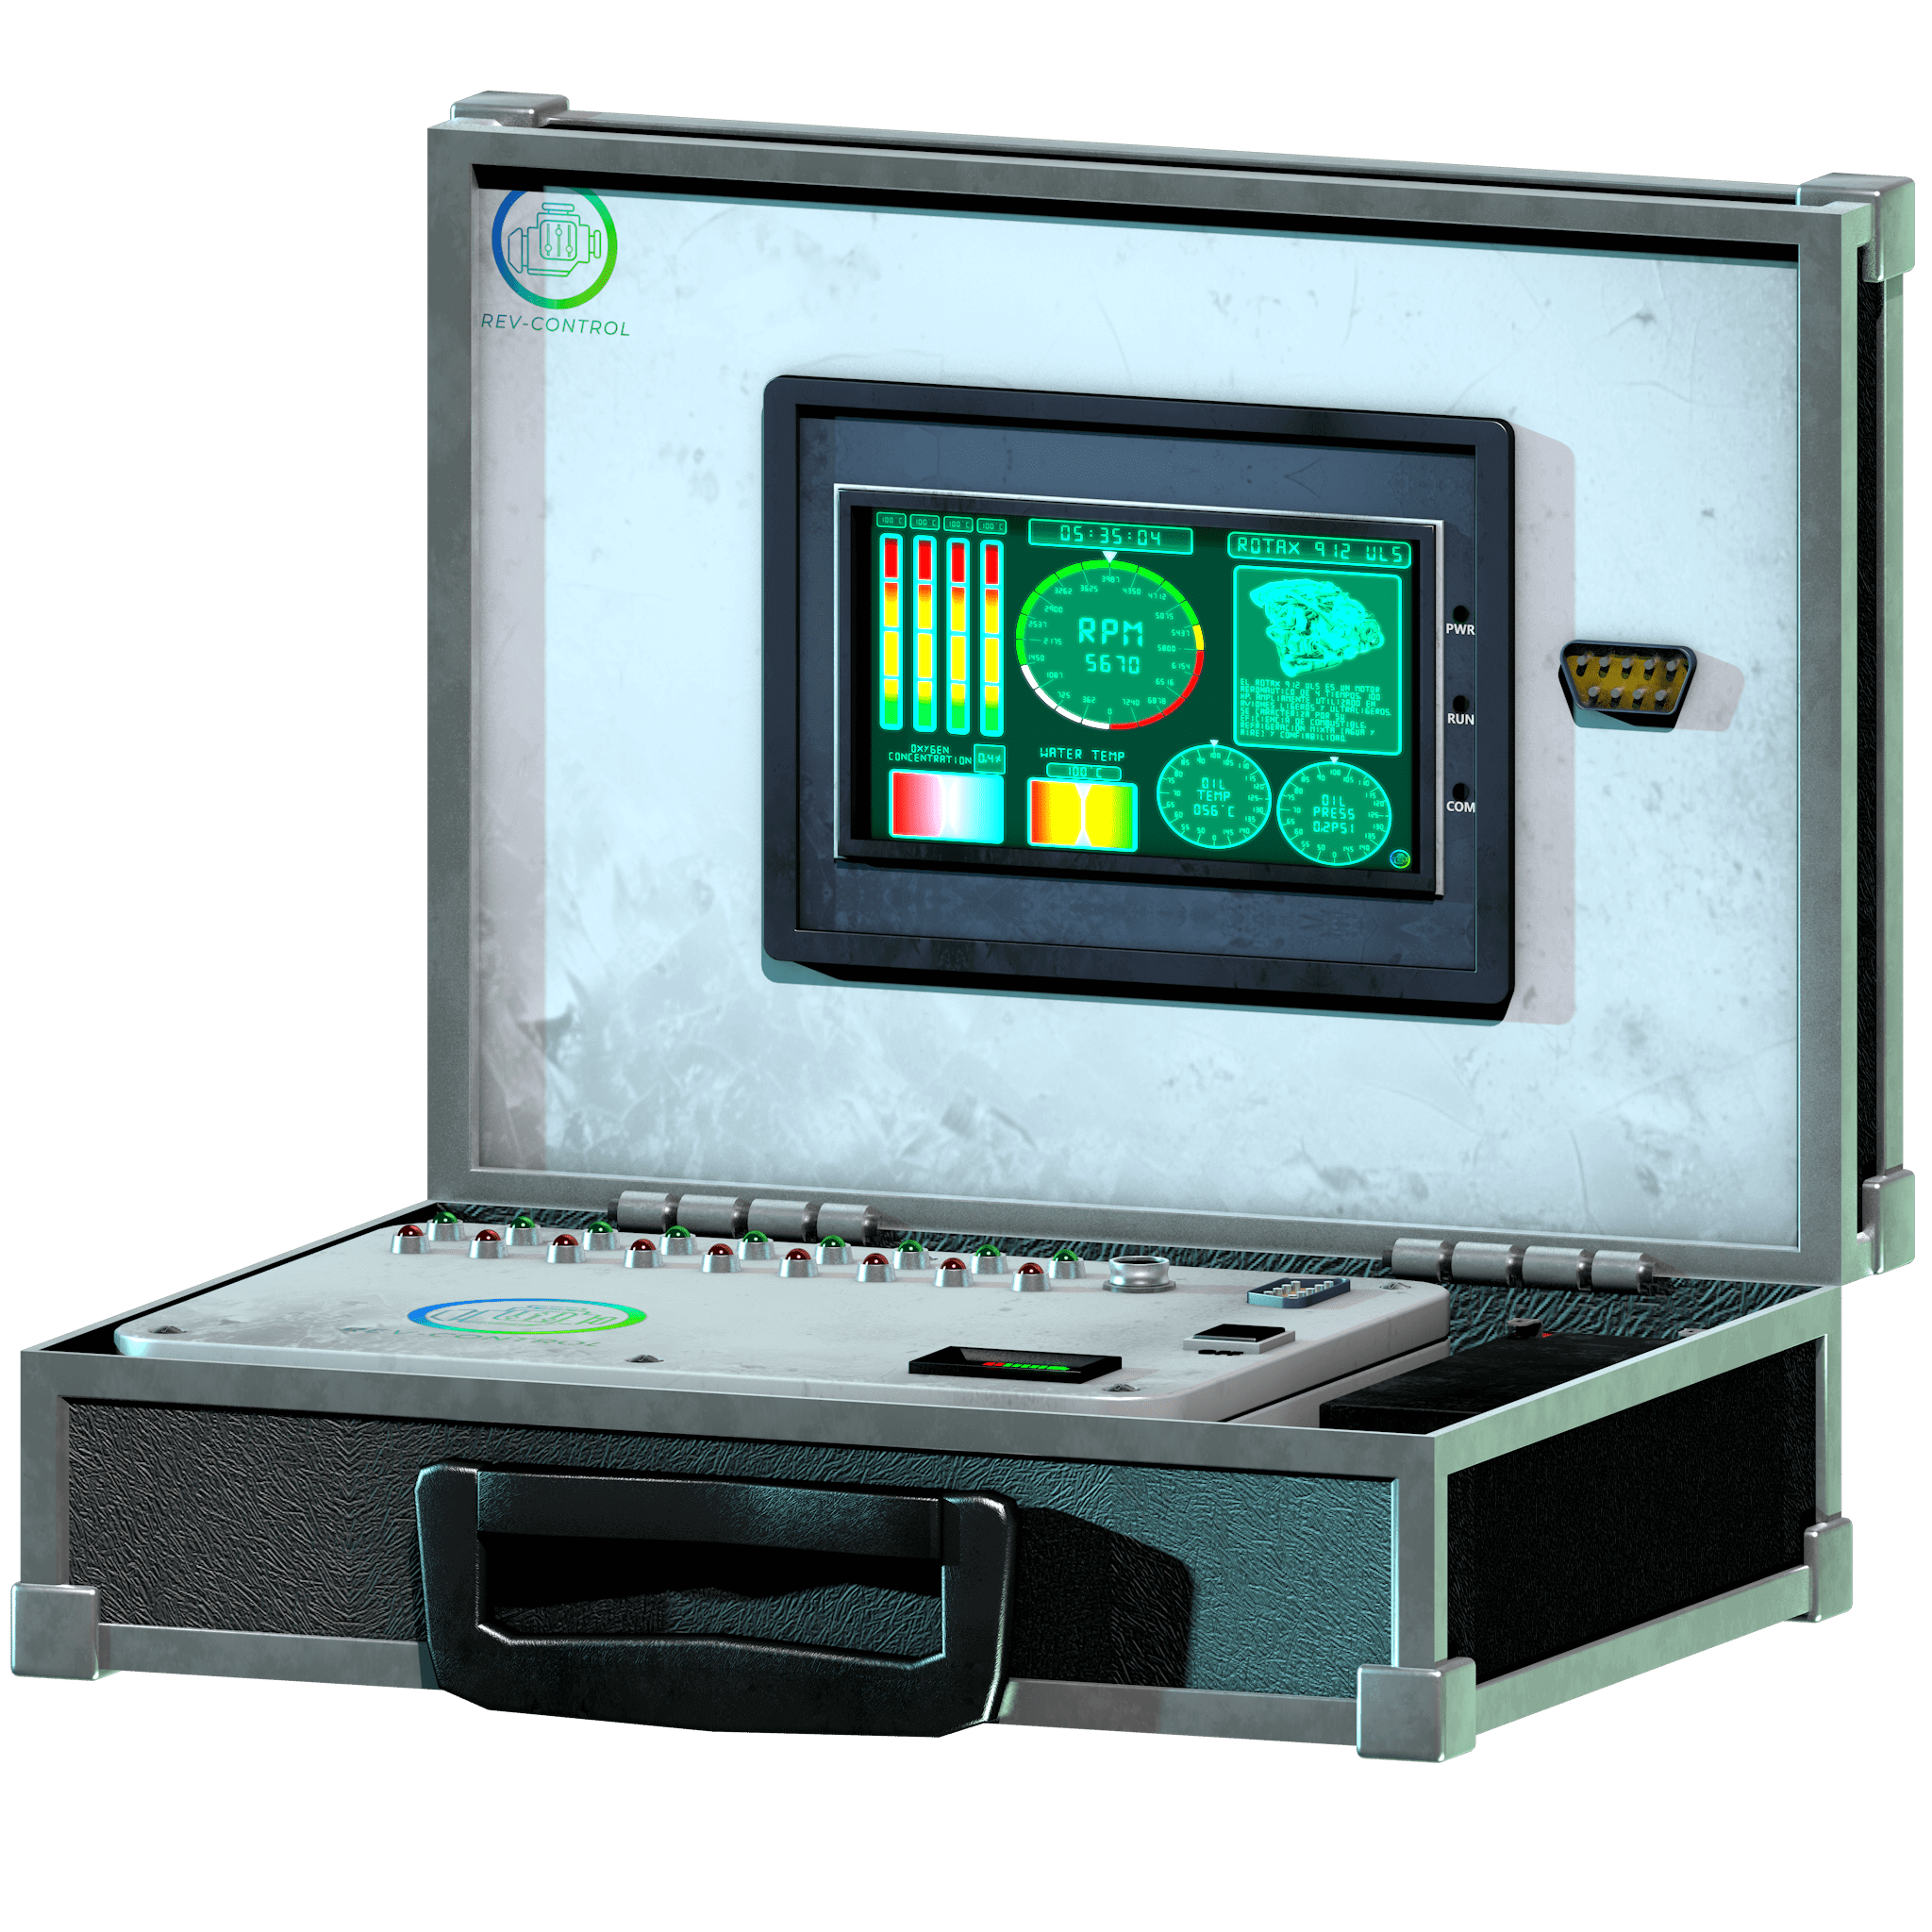
\includegraphics[width=0.6\textwidth]{Imagenes/Monitor y maletin-min.png}
    \caption{Imagen representativa del proyecto REV-CONTROL en funcionamiento.}
    \label{fig:representativa}
\end{figure}

\section{Diagrama en bloques del proyecto}

\begin{figure}[H]
    \centering
    \begin{tikzpicture}[
      block/.style={rectangle, draw, text centered, minimum height=1cm, minimum width=3cm, rounded corners},
      arrow/.style={-{Latex[length=3mm, width=2mm]}, thick},
      node distance=1.5cm
    ]
      
      % Definición de nodos
      \node[block, fill=cyan!30] (motor) {Motor en funcionamiento};
      \node[block, fill=green!30, below=of motor] (sensores) {Sensores de parámetros críticos};
      \node[block, fill=blue!30, below=of sensores] (condicionamiento) {Condicionamiento de señales};
      \node[block, fill=cyan!30, below=of condicionamiento] (lpc845) {Microcontrolador LPC845};
      \node[block, fill=green!30, below=of lpc845] (alarma) {Sistema de alarma};
      \node[block, fill=green!30, right=of lpc845] (monitor) {Monitor Kinseal};

      % Conexiones con flechas
      \draw[arrow] (motor) -- (sensores);
      \draw[arrow] (sensores) -- (condicionamiento);
      \draw[arrow] (condicionamiento) -- (lpc845);
      \draw[arrow] (lpc845) -- (alarma);
      \draw[arrow] (lpc845) -- (monitor);

    \end{tikzpicture}
    \caption{Diagrama en bloques del sistema REV-CONTROL.}
    \label{fig:diagrama_bloques}
\end{figure}

\section{Motor utilizado en el proyecto (ROTAX 912 ULS)}

El \textbf{\href{https://www.flyrotax.com/products/912-uls-s}{Rotax 912 ULS}} es un motor de cuatro tiempos ampliamente utilizado en aeronaves ligeras, vehículos todoterreno y aplicaciones industriales.  
\begin{itemize}
    \item Configuración: Motor bóxer de 4 cilindros, refrigerado por líquido y aire.  
    \item Cilindrada: 1,352 cm³.  
    \item Potencia: 100 HP (73.5 kW) a 5,800 RPM.  
    \item Alimentación: Sistema de carburadores duales.  
    \item Características destacadas: Alta fiabilidad, bajo peso, eficiencia de combustible y capacidad para operar con gasolina sin plomo.  
    \item Aplicación en el proyecto: Recolección y análisis de datos críticos como temperatura, presión de aceite, proporción aire-combustible y velocidad de rotación.  
\end{itemize}

\begin{figure}[H]
    \centering
    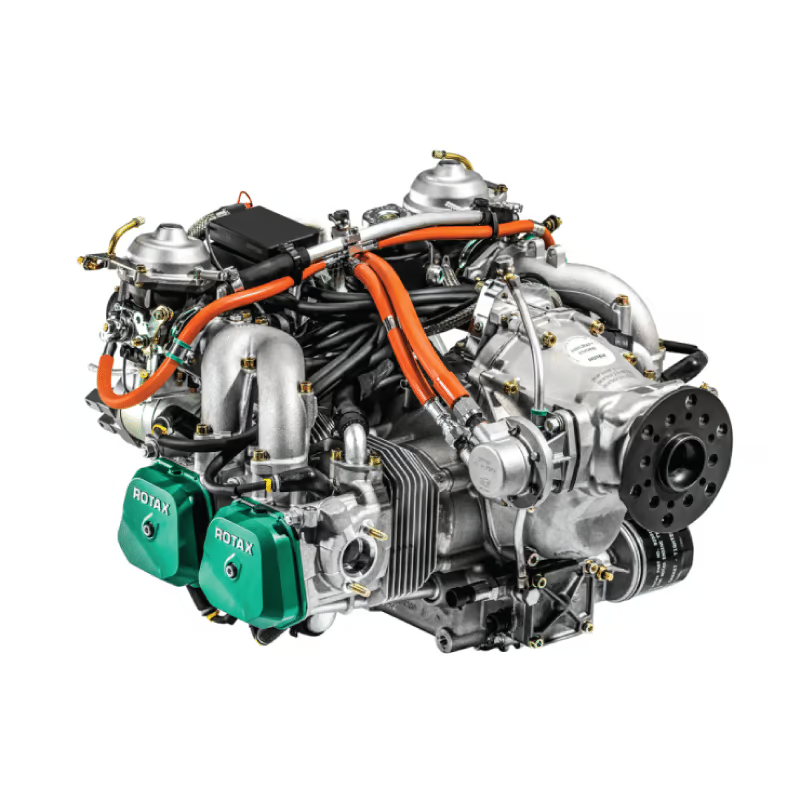
\includegraphics[width=0.8\textwidth]{Imagenes/ROTAX.png}
    \caption{Motor Rotax 912 ULS}
    \label{fig:motor_rotax_912}
\end{figure}


\section{Resultado conseguido}  
El resultado de \textbf{REV-CONTROL} es una herramienta integral para diagnóstico de motores, que ofrece mediciones precisas y en tiempo real de parámetros críticos. Su sistema permite a los técnicos obtener datos detallados de manera clara y sencilla, mejorando la eficacia en las reparaciones y mantenimiento de motores, además de ofrecer un sistema de alarmas para alertar de situaciones críticas en los parámetros monitoreados.



% 5. Software
\chapter{Software}

\section{Códigos significativos}
A continuación se adjunta el código de lectura de pines en \hyperref[adc_code]{ADC} y \hyperref[spi_code]{SPI}:

% Fragmento de código ADC
\lstinputlisting[
    language=C,
    caption=Lectura de ADC, 
    label=adc.code
]{rev-control_adc.c}

% Fragmento de código SPI
\lstinputlisting[
    language=C,
    caption=Lectura de SPI, 
    label=spi.code
]{rev-control_spi.c}
    
    \section{Capturas de interfaces visuales}
        Información
    
    \section{Estructuras de datos}

Esta sección describe las principales estructuras de datos utilizadas para gestionar las lecturas de los sensores y la comunicación SPI en el sistema. Se incluye una descripción de las variables globales, las funciones clave, y las estructuras de configuración para el ADC y el SPI.

\subsection{Variables globales}

Las variables globales se emplean para almacenar la configuración y los resultados de las conversiones ADC y SPI. A continuación, se describen las más importantes:

\begin{itemize}
    \item \textbf{adc\_channel[3]}: Un \textit{array} de 8 bits que define los canales ADC en uso. Cada elemento representa un canal específico:
        \begin{itemize}
            \item \texttt{ADC0\_CH1}: Canal para la concentración de oxígeno.
            \item \texttt{ADC0\_CH2}: Canal para las RPM.
            \item \texttt{ADC0\_CH3}: Canal para la presión de aceite.
        \end{itemize}
        
    \item \textbf{channel\_result[3]}: Un \textit{array} de enteros de 16 bits que almacena los resultados de la conversión ADC para cada canal.

    \item \textbf{lambda}, \textbf{oil\_pressure}, \textbf{RPM}: Variables de 16 bits donde se guardan los valores procesados de cada lectura del canal, correspondientes a la concentración de oxígeno, la presión de aceite y las RPM, respectivamente.

    \item \textbf{CS[7]}: Un \textit{array} de enteros de 8 bits que representa los pines de Chip Select (CS) utilizados para manejar distintos dispositivos SPI conectados al sistema.
\end{itemize}

\subsection{Funciones y prototipos principales}

Estas funciones organizan el flujo del programa, facilitando la adquisición y transmisión de datos desde los sensores al sistema:

\begin{itemize}
    \item \textbf{void ADC\_Configuration(void)}: Configura el ADC, activando los canales necesarios y definiendo los parámetros de conversión.

    \item \textbf{void spi\_cs\_low(void)} y \textbf{void spi\_cs\_high(void)}: Controlan el estado de los pines de Chip Select (CS) para habilitar o deshabilitar el dispositivo SPI según sea necesario.

    \item \textbf{float max6675\_get\_temp(void)}: Realiza una lectura de temperatura desde un sensor MAX6675 a través de SPI, devuelve el valor en grados Celsius.
\end{itemize}

\subsection{Estructura de configuración para el SPI}

La estructura \texttt{spi\_transfer\_t} se utiliza para definir los parámetros de la transferencia SPI. Esto organiza la lectura del sensor de temperatura y otros dispositivos conectados:

\begin{itemize}
    \item \texttt{txData}: Puntero a los datos que se van a transmitir (NULL si no se envían datos).
    \item \texttt{rxData}: Puntero a los datos recibidos en la transferencia.
    \item \texttt{dataSize}: Tamaño de la transferencia en bytes (en este caso, 2 bytes).
    \item \texttt{configFlags}: Indicadores de configuración que controlan la finalización de la transferencia y el formato de los datos.
\end{itemize}

\subsection{Estructura de configuración para el ADC}

La estructura \texttt{adc\_conv\_seq\_config\_t} define el modo de conversión y los canales activos para el ADC. Los campos principales son:

\begin{itemize}
    \item \texttt{channelMask}: Máscara de bits que activa los canales especificados en el ADC.
    \item \texttt{triggerMask}: Define el disparo de conversión, ya sea en modo automático o por software.
    \item \texttt{interruptMode}: Configura las interrupciones que se activan cuando la conversión en un canal finaliza.
\end{itemize}

Estas estructuras de datos, variables y funciones permiten un manejo organizado y eficiente de las lecturas y configuraciones de los sensores en el sistema embebido.

 

    

% 6. Sistema embebido
\chapter{Sistema embebido}
\section{Microcontroladores y/o microprocesadores utilizados}
Información

\section{Placas de desarrollo}
Información

\section{Software utilizados para el desarrollo}
Información

\section{Diagrama en bloque de la solución}
Información

\section{Lenguajes de programación usados}
Información

\section{Capturas de códigos significativos}
Información

\section{Especificación de periféricos utilizados}
Información

\section{Estructuras de datos}
Información

% 7. Electrónica
\chapter{Electrónica}
\section{Diagrama en bloque de las partes}
Información

\section{Software usado para el desarrollo de esquemáticos y PCB}
Información

\section{Esquemático de cada bloque}
Información

\section{PCB de cada bloque}
Información

\section{Modelo 3D de cada PCB}
Información

\section{Especificaciones sobre fuentes de alimentación y potencias}
Información

\section{Especificaciones técnicas de los componentes}
Información

% 8. Estructura
\chapter{Estructura}
\section{Diagrama general de la estructura}
Información

\section{Software de diseño utilizado}
Información

\section{Descripción de cada parte de la estructura}
Información

\section{Imágenes exportadas de los diseños}
Información

% 9. Anexo
\begin{appendix}
   \chapter{Apéndice A: Esquemáticos}
    El circuito Rev-Control Version 2.6 es un sistema de monitoreo y control de parámetros de un motor, diseñado para la medición y alerta de varias variables como RPM, presión de aceite, temperatura y concentración de oxígeno. Este sistema emplea un microcontrolador LPC845 para gestionar las entradas y salidas de los sensores y se conecta mediante un puerto micro-USB. Utiliza múltiples termocuplas, termistores y sensores específicos conectados a través de amplificadores para cada medición.\\

\begin{enumerate}
    \item \textbf{Microcontrolador LPC845}: Procesa las señales y controla el encendido de alertas. Cuenta con múltiples pines asignados a diferentes sensores y señales de salida.

    \item \textbf{Sensores de Temperatura - Termocuplas (MAX6675)}: Las termocuplas están distribuidas en varias posiciones del sistema para medir temperaturas en puntos específicos, con salidas gestionadas a través de los pines PIO0 del microcontrolador.

    \item \textbf{Sensores de Temperatura - Termistores (MAX31865)}: El MAX31865 convierte las señales de los termistores en datos procesables para el microcontrolador, permitiendo mediciones precisas en otras partes del sistema.

    \item \textbf{Sensor de Presión de Aceite}: Este sensor, conectado a los pines PIO0\_23 y PIO0\_01 del microcontrolador, mide la presión de aceite en el motor, operando en un rango de hasta 7 bar. Permite monitorear la lubricación adecuada del motor, activando alertas en caso de lecturas fuera del rango establecido.

    \item \textbf{Sonda Lambda (\%O2)}: Utiliza el amplificador operacional \textbf{LM358} para ajustar la señal de entrada de la sonda, que mide el nivel de oxígeno en los gases de escape. Indicadores visuales muestran el estado de la medición.

    \item \textbf{Regulador de Voltaje (LD1117D12)}: Proporciona una salida de 3.3V para alimentar componentes de bajo voltaje, asegurando una distribución estable de energía en el sistema.

    \item \textbf{Placa Step Down Regulada a 5V}: Regula la alimentación de 12V a 5V para los componentes que requieren esta tensión, proporcionando una fuente de energía estable y eficiente.

    \item \textbf{Potenciómetro y Resistencias}: Utilizados para calibrar y ajustar las señales de algunos sensores, como la señal de RPM.
\end{enumerate}


    \begin{landscape}
        \begin{sidewaysfigure}
            \centering
            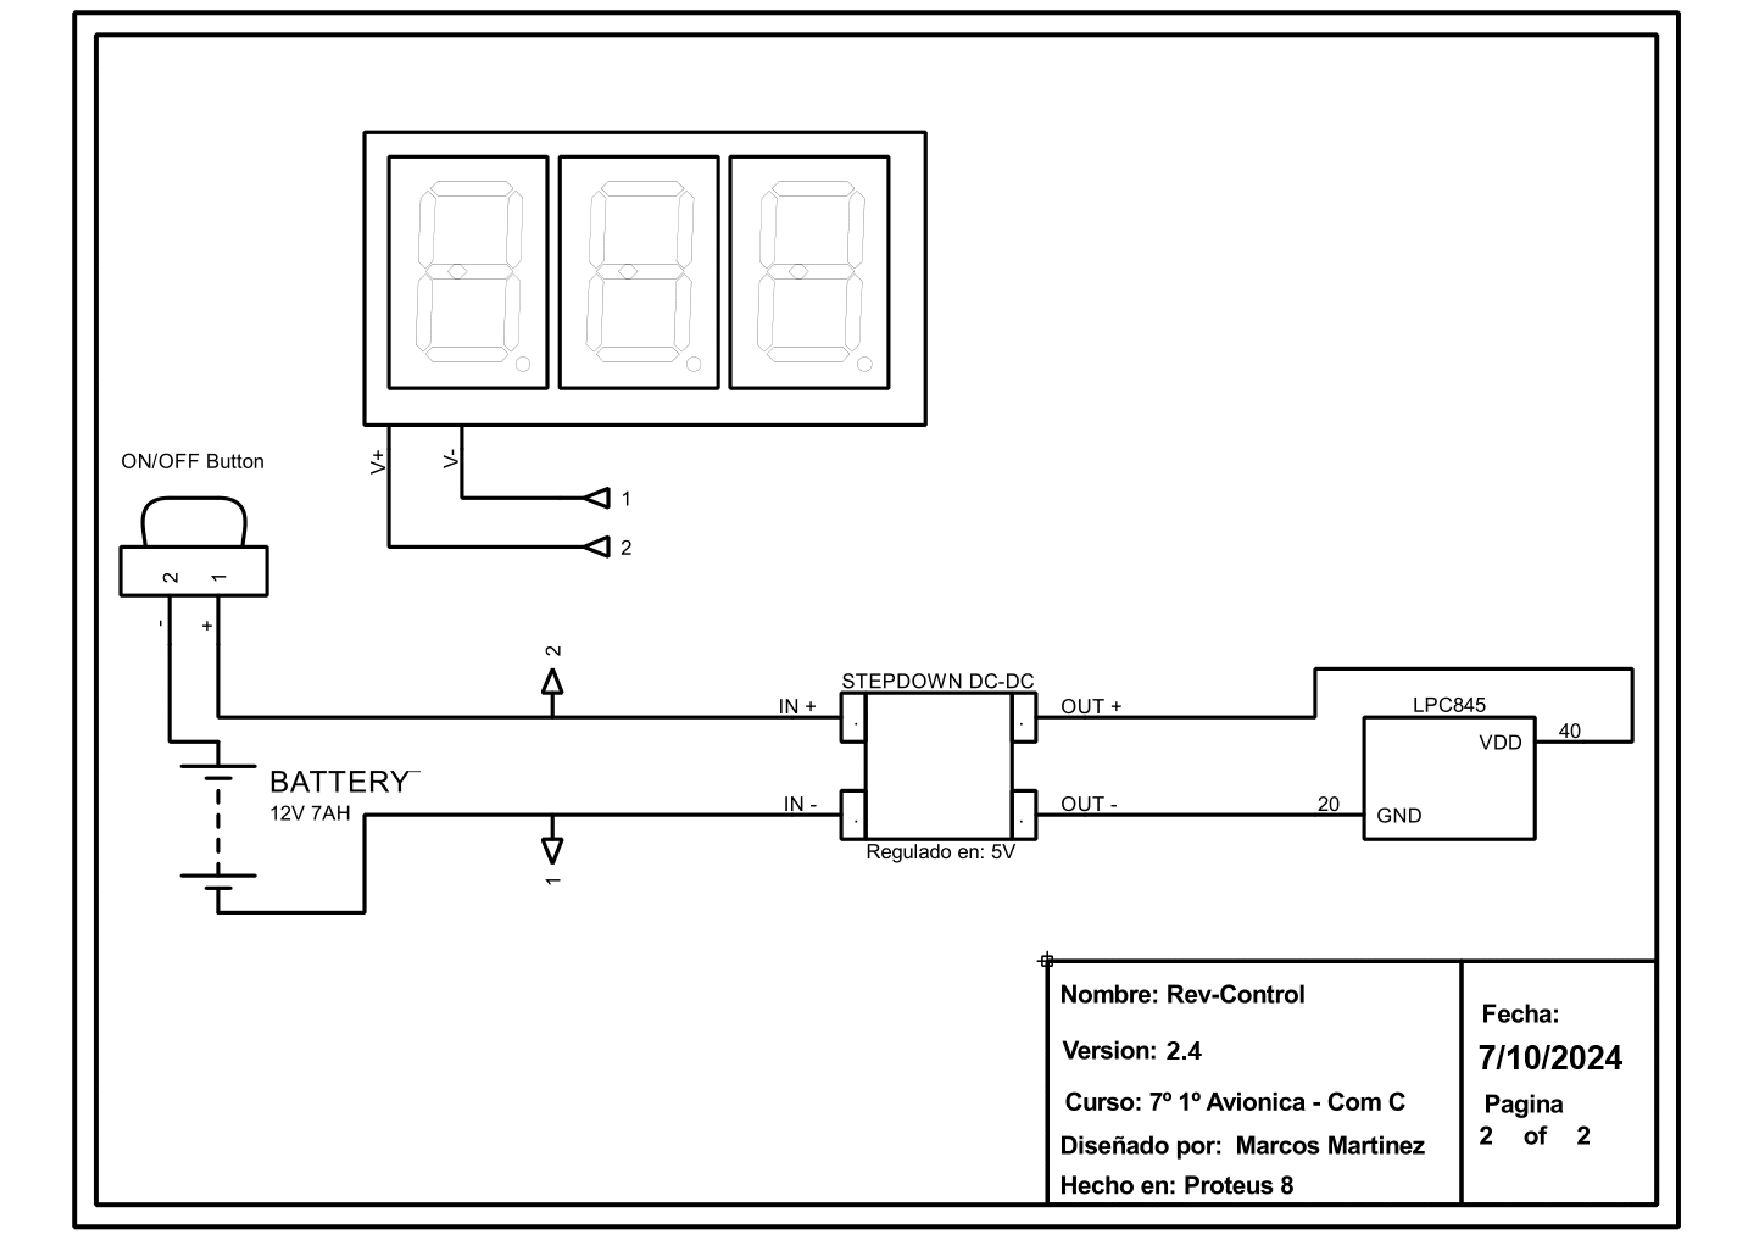
\includegraphics[angle=270, width=\textwidth, keepaspectratio]{Anexo-A Bloque/Rev- Control Version 2.4 Parte 2.pdf}
            \caption{Control Version 2.4 Parte 2}
            \label{fig:A_1}
        \end{sidewaysfigure}
        
        \newpage
        
        \begin{sidewaysfigure}
            \centering
            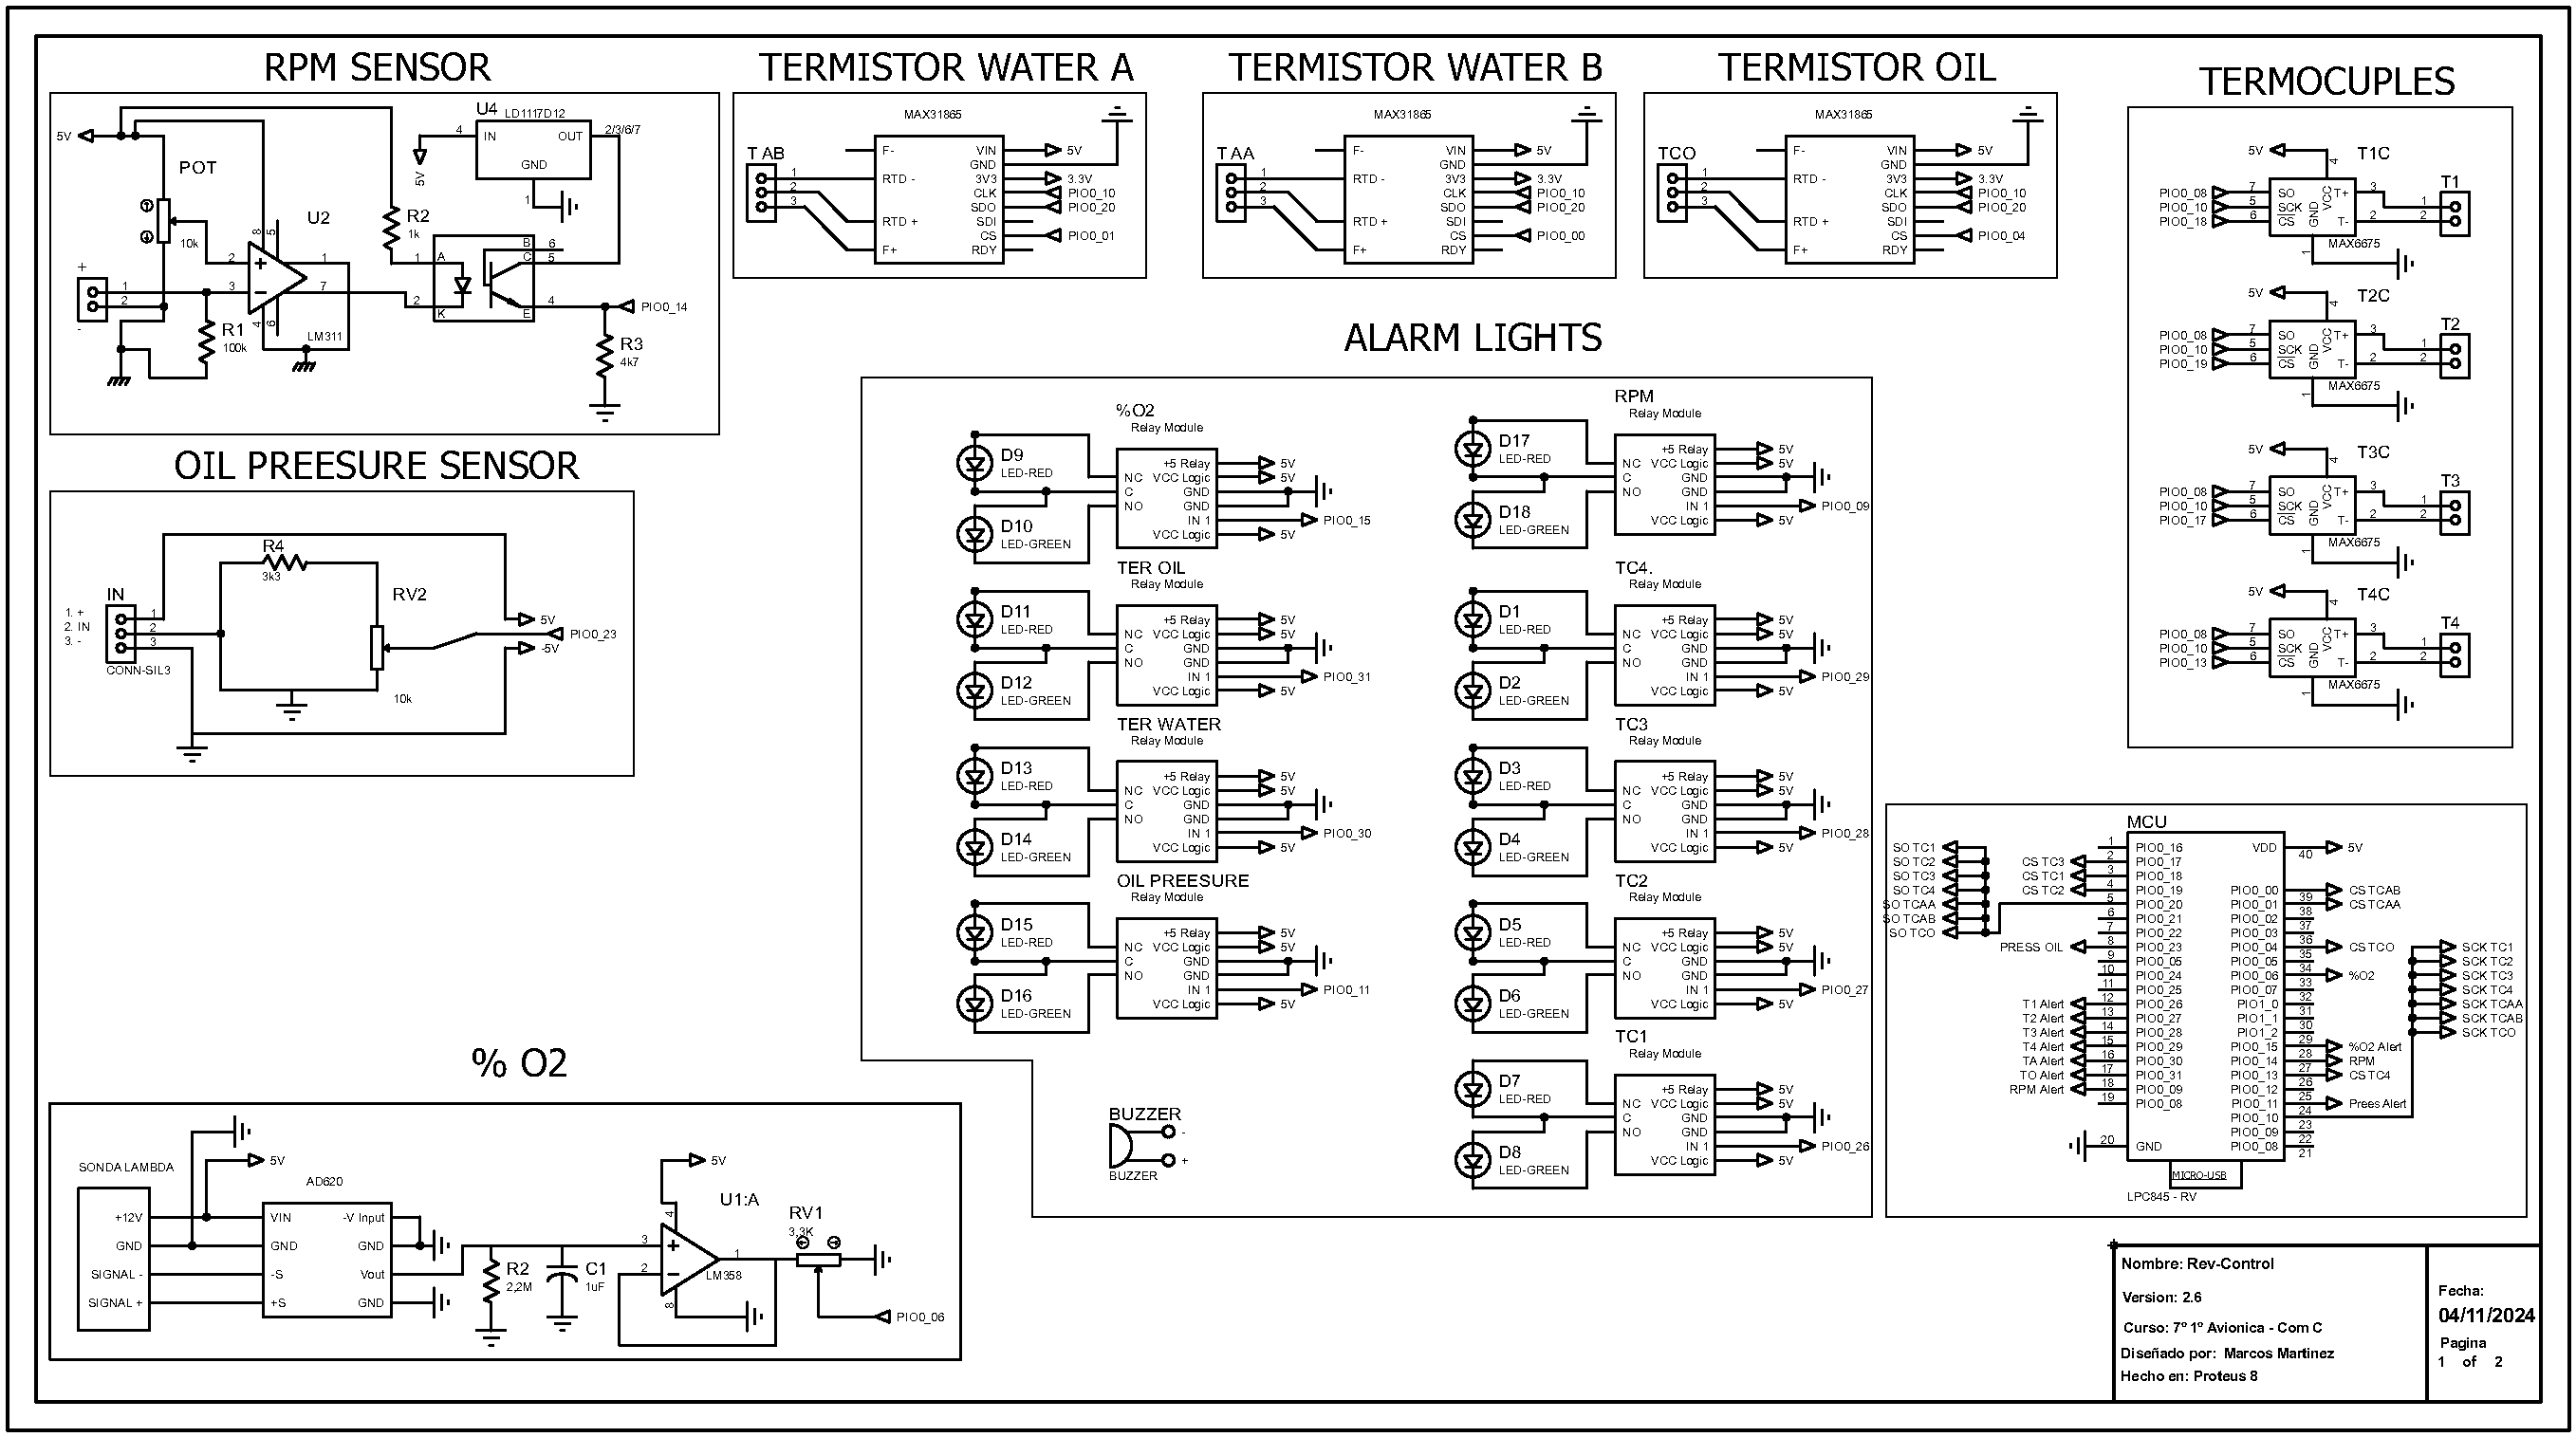
\includegraphics[angle=270, width=\textwidth, keepaspectratio]{Anexo-A Bloque/REV-CONTROL version 2.6.PDF}
            \caption{Control Version 2.6}
            \label{fig:A_2}
        \end{sidewaysfigure}
        
    \end{landscape}
   \chapter{Apéndice B: Documentación-ROTAX}
    La información presentada aquí es el certificado de Aeronavegabilidad y documentación técnica del motor trabajado en este proyecto (Motor ROTAX 912 ULS). Para presentar la bases de información que utilizamos para este proyecto respecto a los parámetros. A continuación se va adjuntar las fuentes de adquisición de dichos documentos y fragmentos de estos mismos:
    
\begin{itemize}
    \item Certificado de Aeronavegabilidad: 
    \hyperlink{certificado-aeronavegabilidad}{-Salto a página-}
    \href{https://www.seguridadaerea.gob.es/sites/default/files/HD%20TC286-I%20r8.pdf}{www.seguridadaerea.gob.es}
    \hfill
     % Enlace directo a la primera página del certificado
    
    \item Documentación Técnica:
    \href{https://www.flyrotax.com/p/service/technical-documentation}{www.flyrotax.com} 

    \begin{itemize}
        \item SERVICE INSTRUCTION - PAC (Pag. 8) 
        \hyperlink{service-instruction-pag8}{-Salto a página-} % Enlace directo a la página 8 en el documento
    \end{itemize}

    \begin{itemize}
        \item MAINTENANCE MANUAL LINE (Pag. 89-90,91-92,88,100,101-103)
        \hyperlink{maintenance-manual-pag91-92}{-Salto a página-} % Enlace directo a la página 91-92 en el documento
    \end{itemize}

    \begin{itemize}
        \item OPERATORS MANUAL LINE (Pag. x)(Pag. 28-29,32)
        \hyperlink{operators-manual1}{-Salto a página-} 
    \end{itemize}

    \begin{itemize}
        \item USER MANUAL (Pag. 35-37) 
        \hyperlink{user-manual}{-Salto a página-} 
    \end{itemize}

    \begin{itemize}
        \item INSTALLATION MANUAL (Pag. 157-158) 
        \hyperlink{manual de instalacion}{-Salto a página-} 
    \end{itemize}
\end{itemize}

% Insertar el PDF completo a continuación de la descripción
\begin{landscape}
    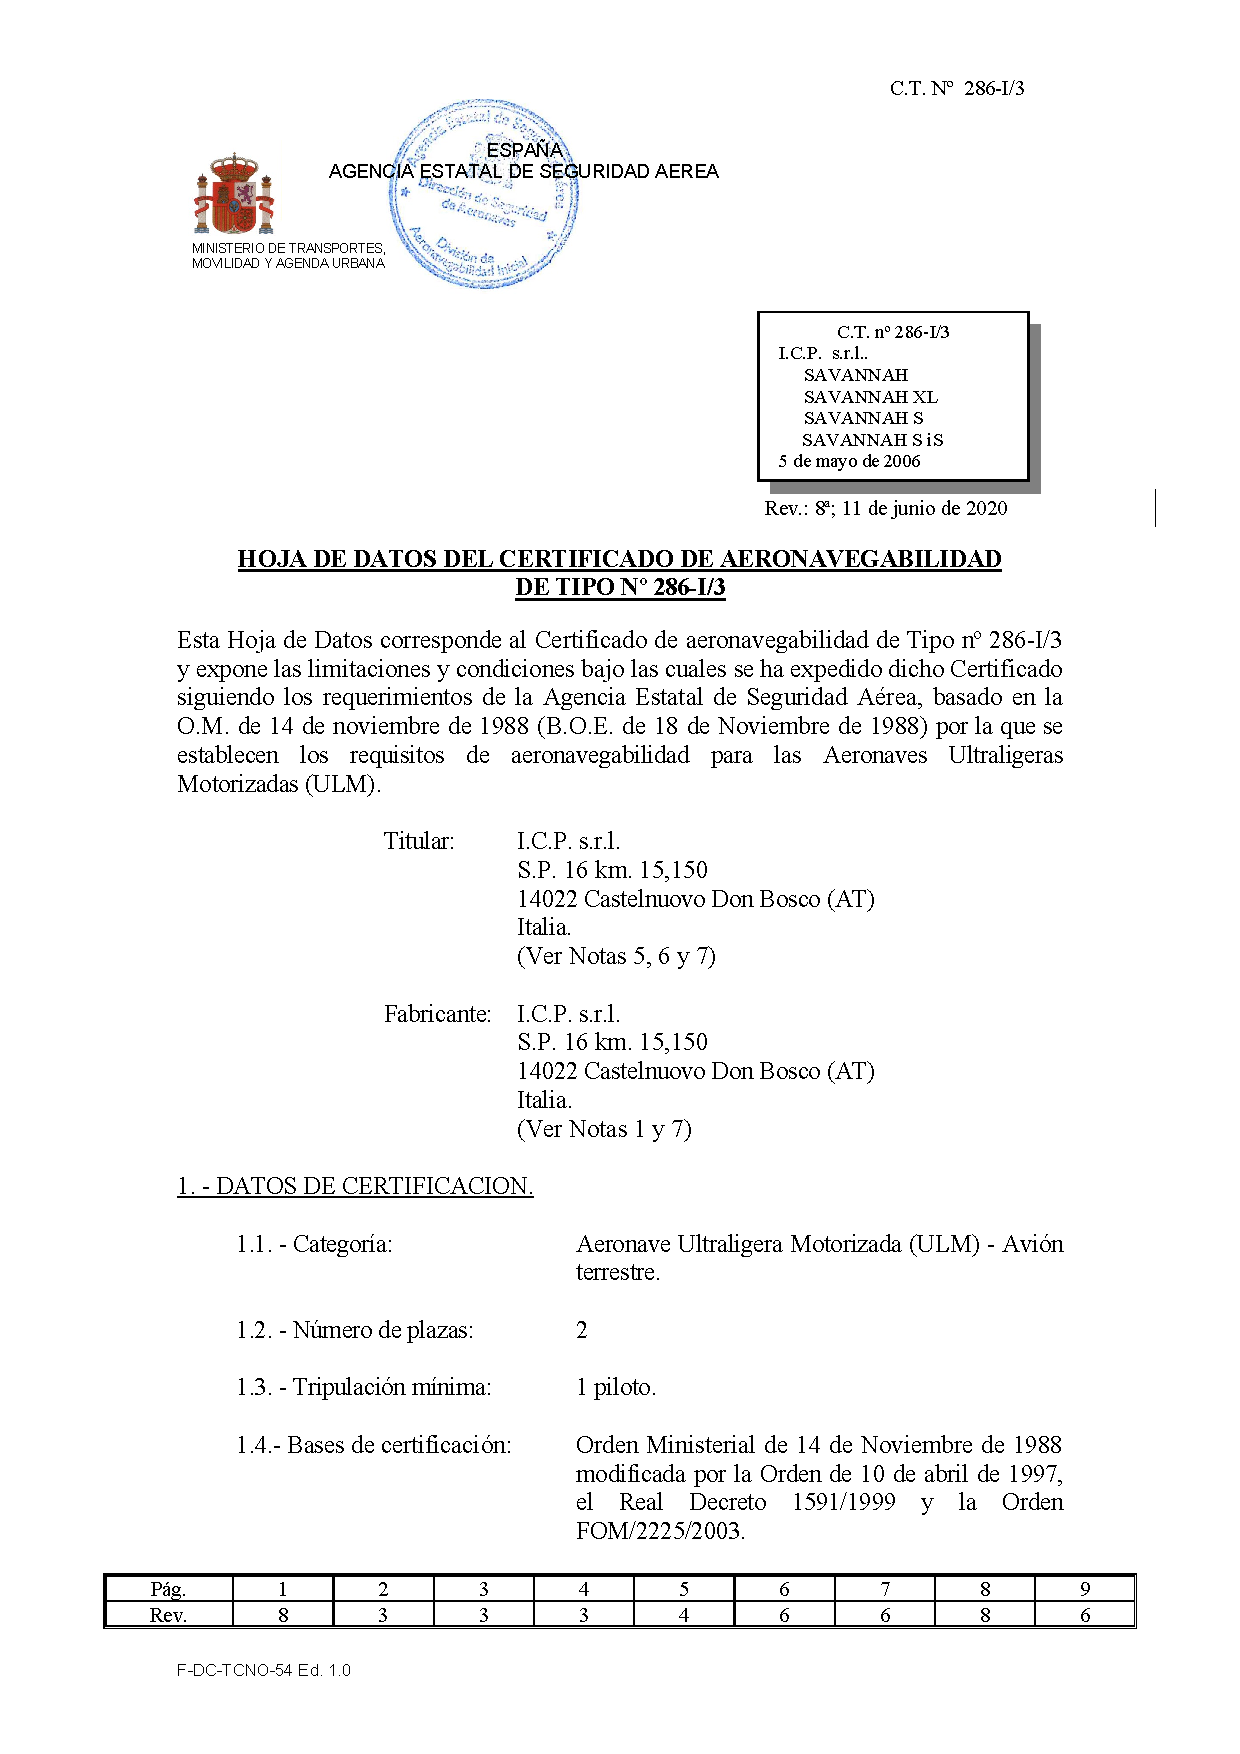
\includepdf[pages=1-2, scale=0.9, pagecommand={\hypertarget{certificado-aeronavegabilidad}{}}]{Anexo-B Bloque/HD TC286-I r8.pdf}
\end{landscape}

\begin{landscape}
    \includepdf[pages=6, scale=0.9, pagecommand={\hypertarget{service-instruction-pag8}{}}]{Anexo-B Bloque/SI-PAC-027.pdf}
\end{landscape}

\begin{landscape}
    
\includepdf[pages={89-90,91-92,88,100,101,102,103}, scale=0.9, pagecommand={\hypertarget{maintenance-manual-pag91-92}{}}]{Anexo-B Bloque/Maintenance Manual Line for Engine Type 912 Series Edition 4 Revision 1.pdf}
\end{landscape}

\begin{landscape}
    \includepdf[pages={28-29,32}, scale=0.9, pagecommand={\hypertarget{operators-manual1}{}}]{Anexo-B Bloque/OM_912 Series_ED4_R1.pdf}
\end{landscape}

\begin{landscape}
    \includepdf[pages={35-37,28}, scale=0.9, pagecommand={\hypertarget{user-manual}{}}]{Anexo-B Bloque/Manual_Usuario_912.pdf}
\end{landscape}

\begin{landscape}
    \includepdf[pages={157-158}, scale=0.9, pagecommand={\hypertarget{manual de instalacion}{}}]{Anexo-B Bloque/IM_912_Series_Ed3_R0.pdf}
\end{landscape}



\end{appendix}



\end{document}